\documentclass[aspectratio=169,11pt,t]{beamer}
\usepackage[T1]{fontenc}
\usepackage{mathptmx}
\usepackage[scaled=.92]{helvet}
\usepackage{booktabs,tikz}
\usetikzlibrary{arrows.meta,shapes.geometric}
\definecolor{gradOrange}{HTML}{F07F3C}
\definecolor{gradPurple}{HTML}{B84FC2}
\definecolor{iiscOrange}{gray}{0.45}
\definecolor{iiscPurple}{gray}{0.1}
\definecolor{accP}{HTML}{5F4B6B}
\definecolor{accA}{HTML}{C58A63}
\setbeamercolor{background canvas}{bg=white!99!black}
\setbeamercolor{structure}{fg=iiscPurple}
\setbeamercolor{itemize item}{fg=iiscOrange}
\setbeamercolor{itemize subitem}{fg=iiscPurple}
\setbeamerfont{frametitle}{series=\bfseries,size=\LARGE}
\setbeamertemplate{navigation symbols}{}
\setbeamertemplate{itemize item}[square]
% title pinned to the top of the slide
\setbeamertemplate{frametitle}{\vskip1.1ex{\color{black}\sffamily\bfseries\LARGE\insertframetitle}\par\vskip1.2ex}
\setbeamertemplate{background}{\vbox to\paperheight{\vfill\hbox to\paperwidth{%
  \tikz[baseline=0]\shade[left color=gradOrange,right color=gradPurple] (0,0) rectangle (\paperwidth,.16);}}}
\setbeamertemplate{footline}{\hfill{\color{black!35}\fontsize{7}{8}\selectfont\insertframenumber/\inserttotalframenumber}\hspace*{.85cm}\vskip4.6ex}
\setbeamersize{text margin left=1.6cm,text margin right=1.6cm}
% ---- extras needed by the content
\usepackage{amsmath,amssymb}
\usepackage[ruled,vlined,linesnumbered]{algorithm2e}
\SetAlFnt{\scriptsize}\SetAlCapFnt{\scriptsize}
\newcommand{\Agree}{93.8}
\newcommand{\AllGunsBusyPlans}{66}
\newcommand{\BattMilp}{71.1}
\newcommand{\BattRl}{63.5}
\newcommand{\BestEpoch}{180}
\newcommand{\BusyHalfHiM}{26.0}
\newcommand{\BusyHalfLoM}{0.6}
\newcommand{\BusyHalfMedM}{10.3}
\newcommand{\BusyHiM}{21.8}
\newcommand{\BusyHiR}{21.9}
\newcommand{\BusyLoM}{6.2}
\newcommand{\BusyLoR}{6.6}
\newcommand{\BusyMedM}{23.3}
\newcommand{\BusyMedR}{23.9}
\newcommand{\ChargeMilp}{24.8}
\newcommand{\ChargeRl}{22.0}
\newcommand{\ComVanHigh}{98.1}
\newcommand{\ComVanTL}{100.0}
\newcommand{\ComVanThetaR}{0.34}
\newcommand{\ComVanWait}{129}
\newcommand{\DeltaComOne}{146}
\newcommand{\EeightBatt}{$-$17.1}
\newcommand{\FleetMilp}{43.9}
\newcommand{\FleetRl}{41.6}
\newcommand{\GapMean}{0.85}
\newcommand{\GapMed}{0.76}
\newcommand{\GapOpt}{0.92}
\newcommand{\GunMaxM}{91.4}
\newcommand{\GunPninetyM}{34.6}
\newcommand{\GunUtilLong}{7.8}
\newcommand{\GunUtilMilp}{12.8}
\newcommand{\GunUtilRl}{13.3}
\newcommand{\GunUtilShort}{19.4}
\newcommand{\GunsNeverM}{29.0}
\newcommand{\IdleGunsMilp}{7.0}
\newcommand{\IdleGunsRl}{6.1}
\newcommand{\NComVan}{103}
\newcommand{\NInf}{51}
\newcommand{\NInst}{560}
\newcommand{\NNoPlan}{35}
\newcommand{\NOpt}{277}
\newcommand{\NPaired}{474}
\newcommand{\NTL}{197}
\newcommand{\NValidM}{474}
\newcommand{\NValidR}{500}
\newcommand{\NVansM}{1040}
\newcommand{\NVansR}{985}
\newcommand{\OffpeakHigh}{19.8}
\newcommand{\OmegaHiComHighM}{$-$0.3}
\newcommand{\OmegaHiComHighR}{$-$0.6}
\newcommand{\PMLoPersHighM}{+4.7}
\newcommand{\PMLoPersLowM}{+16.9}
\newcommand{\Params}{765\,858}
\newcommand{\PayCom}{335}
\newcommand{\PayPers}{352}
\newcommand{\PeakGunsHundredM}{17.5}
\newcommand{\PeakGunsM}{12.9}
\newcommand{\PeakGunsR}{13.1}
\newcommand{\PeakLabelHigh}{38.7}
\newcommand{\PeakLabelShare}{32.5}
\newcommand{\PercCom}{582}
\newcommand{\PercPers}{662}
\newcommand{\PressCutHi}{0.69}
\newcommand{\PressCutLo}{0.17}
\newcommand{\PressLoadHi}{20}
\newcommand{\PressLoadLo}{5}
\newcommand{\PressWinMax}{62}
\newcommand{\PressWinMin}{46}
\newcommand{\QShareComM}{91.7}
\newcommand{\QShareComR}{94.2}
\newcommand{\QSharePoorM}{76.0}
\newcommand{\QSharePoorR}{72.8}
\newcommand{\QUserComM}{74.2}
\newcommand{\QUserComR}{71.1}
\newcommand{\QUserPoorM}{49.2}
\newcommand{\QUserPoorR}{47.2}
\newcommand{\QueueAllHiM}{5.52}
\newcommand{\QueueAllHiR}{7.65}
\newcommand{\QueueAllLoM}{0.03}
\newcommand{\QueueAllLoR}{0.12}
\newcommand{\QueueAllMedM}{0.26}
\newcommand{\QueueAllMedR}{0.67}
\newcommand{\QueueNeedCom}{20}
\newcommand{\QueueNeedComZero}{197}
\newcommand{\QueuedHiM}{30.3}
\newcommand{\QueuedLoM}{0.5}
\newcommand{\QueuedM}{7.7}
\newcommand{\QueuedMedM}{3.1}
\newcommand{\QueuedR}{10.0}
\newcommand{\RLGunBaseDemandHigh}{10.6}
\newcommand{\RLGunBaseDemandLow}{15.8}
\newcommand{\RLGunBaseGunsFour}{15.8}
\newcommand{\RLGunBaseGunsOne}{11.2}
\newcommand{\RLGunBasePowerEleven}{9.3}
\newcommand{\RLGunBasePowerFortyFour}{15.8}
\newcommand{\RLGunDemandHigh}{13.2}
\newcommand{\RLGunDemandLow}{12.0}
\newcommand{\RLGunGunsFour}{8.0}
\newcommand{\RLGunGunsOne}{21.0}
\newcommand{\RLGunPowerEleven}{15.5}
\newcommand{\RLGunPowerFortyFour}{8.1}
\newcommand{\RLLostDemandHigh}{79}
\newcommand{\RLLostDemandLow}{0}
\newcommand{\RLLostGunsFour}{0}
\newcommand{\RLLostGunsOne}{68}
\newcommand{\RLLostPowerEleven}{102}
\newcommand{\RLLostPowerFortyFour}{0}
\newcommand{\RLNewDemandHigh}{0}
\newcommand{\RLNewDemandLow}{39}
\newcommand{\RLNewGunsFour}{9}
\newcommand{\RLNewGunsOne}{0}
\newcommand{\RLNewPowerEleven}{0}
\newcommand{\RLNewPowerFortyFour}{32}
\newcommand{\RLQHighBaseDemandHigh}{7.54}
\newcommand{\RLQHighBaseDemandLow}{8.78}
\newcommand{\RLQHighBaseGunsFour}{8.78}
\newcommand{\RLQHighBaseGunsOne}{5.90}
\newcommand{\RLQHighBasePowerEleven}{6.73}
\newcommand{\RLQHighBasePowerFortyFour}{8.78}
\newcommand{\RLQHighDemandHigh}{7.38}
\newcommand{\RLQHighDemandLow}{8.24}
\newcommand{\RLQHighGunsFour}{1.92}
\newcommand{\RLQHighGunsOne}{12.28}
\newcommand{\RLQHighPowerEleven}{3.61}
\newcommand{\RLQHighPowerFortyFour}{7.09}
\newcommand{\RLVanPDemandHigh}{$-$0.8}
\newcommand{\RLVanPDemandLow}{$-$0.6}
\newcommand{\RLVanPGunsFour}{$-$1.4}
\newcommand{\RLVanPGunsOne}{+10.6}
\newcommand{\RLVanPPowerEleven}{+52.4}
\newcommand{\RLVanPPowerFortyFour}{$-$6.7}
\newcommand{\RLdZDemandHigh}{+22.19}
\newcommand{\RLdZDemandLow}{$-$21.82}
\newcommand{\RLdZGunsFour}{$-$2.21}
\newcommand{\RLdZGunsOne}{+4.76}
\newcommand{\RLdZPowerEleven}{+20.13}
\newcommand{\RLdZPowerFortyFour}{$-$12.30}
\newcommand{\RlBetter}{28}
\newcommand{\RlOnly}{26}
\newcommand{\RoadMilp}{68.4}
\newcommand{\RoadRl}{68.6}
\newcommand{\SeatsEightSeats}{$-$17.1}
\newcommand{\SeatsMilp}{79.0}
\newcommand{\SeatsRl}{69.4}
\newcommand{\Speed}{1\,172}
\newcommand{\SysMilp}{12.4}
\newcommand{\SysRl}{12.4}
\newcommand{\TabEquity}{$\theta$ 0.0--0.2 & 277 & 509 & 510 & 334 & 607 & 605 \\ $\theta$ 0.2--0.4 & 337 & 646 & 634 & 339 & 594 & 603 \\ $\theta$ 0.4--0.6 & 337 & 675 & 673 & 331 & 560 & 572 \\ $\theta$ 0.6--0.8 & 332 & 691 & 700 & 336 & 559 & 568 \\ $\theta$ 0.8--1.0 & 381 & 646 & 717 & 241 & 425 & 439 \\}
\newcommand{\TabExpCost}{$p^M$ 15 & 471 (1/4) & $-$4.19 & +3.69 & $-$7.80 & $-$3.74 & $-$3.78 \\ $p^M$ 35 & 477 (3/0) & +3.91 & $-$1.39 & +6.53 & +3.64 & +3.73 \\ 3 vans & 441 (0/33) & $-$0.04 & $-$0.53 & +0.20 & +0.02 & +0.09 \\ 7 vans & 487 (13/0) & +0.02 & +0.22 & $-$0.05 & +0.04 & +0.00 \\ 4 seats & 471 (4/7) & +1.08 & +3.03 & +0.26 & +0.91 & +0.88 \\ 8 seats & 471 (0/3) & $-$0.08 & $-$0.28 & +0.06 & $-$0.08 & +0.07 \\ taxi $\omega^1$ 4.5 & 472 (1/3) & $-$2.67 & $-$0.17 & $-$3.80 & $-$2.72 & $-$2.52 \\ taxi $\omega^1$ 7.5 & 475 (3/2) & +2.66 & +0.26 & +3.81 & +2.72 & +2.75 \\ pers. $c^{C,1}$ 7.5 & 473 (1/2) & $-$2.21 & $-$1.15 & $-$2.59 & $-$2.49 & $-$2.46 \\ pers. $c^{C,1}$ 12.5 & 473 (1/2) & +2.08 & +2.75 & +1.84 & +2.45 & +2.38 \\ pers. $\mu^0$ 1.125 & 473 (1/2) & $-$1.35 & $-$0.01 & $-$1.96 & $-$1.28 & $-$1.22 \\ pers. $\mu^0$ 1.875 & 475 (2/1) & +1.33 & $-$0.15 & +2.04 & +1.29 & +1.36 \\ taxi $\mu^0$ 1.125 & 475 (1/0) & $-$6.38 & +0.05 & $-$9.40 & $-$6.31 & $-$6.25 \\ taxi $\mu^0$ 1.875 & 475 (2/1) & +6.43 & +0.06 & +9.47 & +6.34 & +6.33 \\ battery 200 & 476 (3/1) & $-$0.01 & $-$0.40 & +0.19 & $-$0.02 & $-$0.07 \\}
\newcommand{\TabExpPress}{$p^M$ 15 & +16.9 & +4.7 & +0.8 & $-$0.1 & $-$0.76 \\ $p^M$ 35 & $-$7.0 & $-$4.2 & +0.2 & +0.1 & +0.23 \\ 3 vans & $-$0.9 & $-$4.5 & $-$0.4 & $-$0.8 & $-$0.32 \\ 7 vans & +0.9 & +1.0 & $-$0.0 & $-$1.0 & $-$0.12 \\ 4 seats & $-$10.1 & $-$3.7 & $-$0.4 & $-$0.8 & +0.24 \\ 8 seats & +2.6 & $-$0.6 & +0.4 & +0.1 & $-$0.29 \\ taxi $\omega^1$ 4.5 & $-$0.6 & $-$0.6 & $-$0.2 & $-$1.3 & +0.29 \\ taxi $\omega^1$ 7.5 & +0.0 & +0.2 & $-$0.3 & $-$0.6 & $-$0.51 \\}
\newcommand{\TabExpWho}{$p^M$ 15 & +11.6 & +0.6 & +4.6 & $-$0.4 & +4.6 & +4.0 & +5.1 & +3.8 \\ $p^M$ 35 & $-$6.4 & +0.0 & $-$5.6 & +0.3 & $-$1.4 & $-$3.7 & $-$3.6 & $-$2.1 \\ 3 vans & $-$2.0 & $-$0.1 & $-$0.5 & +0.1 & +25.0 & +0.2 & +0.1 & $-$0.4 \\ 7 vans & +0.6 & $-$0.0 & +0.3 & $-$0.0 & $-$12.2 & $-$0.4 & $-$0.3 & +0.1 \\ 4 seats & $-$8.2 & $-$0.1 & +0.5 & +0.2 & +6.6 & +12.8 & $-$14.9 & $-$1.3 \\ 8 seats & +1.7 & +0.1 & +0.5 & $-$0.0 & $-$0.9 & $-$17.1 & +2.6 & +0.2 \\ taxi $\omega^1$ 4.5 & $-$0.3 & $-$0.0 & +0.8 & +0.0 & $-$0.2 & +0.0 & $-$0.0 & $-$0.1 \\ taxi $\omega^1$ 7.5 & $-$0.3 & $-$0.0 & +0.3 & +0.0 & +0.4 & $-$1.1 & $-$1.0 & $-$0.0 \\ pers. $c^{C,1}$ 7.5 & $-$5.9 & +0.1 & $-$2.9 & +0.2 & $-$1.0 & $-$3.8 & $-$3.5 & $-$1.9 \\ pers. $c^{C,1}$ 12.5 & +9.5 & $-$0.1 & +5.0 & $-$0.3 & +3.8 & +2.0 & +2.6 & +2.3 \\ pers. $\mu^0$ 1.125 & $-$0.1 & $-$0.1 & +1.1 & +0.0 & $-$0.1 & $-$0.1 & $-$0.1 & +0.0 \\ pers. $\mu^0$ 1.875 & $-$1.0 & $-$0.0 & +0.5 & +0.0 & $-$0.2 & $-$0.7 & $-$0.7 & $-$0.3 \\ taxi $\mu^0$ 1.125 & $-$0.3 & +0.0 & +0.4 & +0.0 & +0.1 & $-$0.5 & $-$0.5 & $-$0.1 \\ taxi $\mu^0$ 1.875 & $-$0.1 & +0.0 & +1.0 & +0.0 & +0.1 & $-$0.3 & $-$0.4 & $-$0.1 \\ battery 200 & $-$1.4 & $-$0.0 & +1.4 & +0.0 & $-$1.0 & +0.4 & $-$17.1 & $-$0.1 \\}
\newcommand{\TabInfraFam}{C1 & 1236 & 8.0 & 8.5 & 9.4 & 11.3 & 43.6 & 42.5 & 94.6 & 79.6 & 21.0 & 17.6 \\ C2 & 3390 & 3.0 & 3.1 & 8.3 & 8.9 & 38.0 & 36.2 & 92.1 & 78.2 & 21.5 & 16.6 \\ R1 & 230 & 26.9 & 27.7 & 5.7 & 15.6 & 46.7 & 44.8 & 50.6 & 45.9 & 23.3 & 21.5 \\ R2 & 1000 & 9.2 & 9.6 & 4.9 & 14.4 & 41.8 & 40.4 & 93.8 & 80.6 & 19.6 & 15.8 \\ RC1 & 240 & 30.0 & 31.4 & 6.3 & 16.7 & 48.6 & 41.0 & 41.3 & 37.2 & 14.1 & 11.2 \\ RC2 & 960 & 10.7 & 11.0 & 7.4 & 12.0 & 47.8 & 44.8 & 81.0 & 75.2 & 18.4 & 16.5 \\}
\newcommand{\TabPress}{low & 46.9 & 23.4 & 9.4 & 0.0 & 0.0 & 0.00 & 0.02 & 0.04 & 0.16 \\ medium & 31.5 & 17.1 & 4.8 & 0.0 & 0.0 & 0.06 & 0.12 & 0.33 & 0.89 \\ high & 21.6 & 16.6 & 2.6 & 3.4 & 3.3 & 1.67 & 1.45 & 7.04 & 10.49 \\}
\newcommand{\TabQueueShare}{personal & 25.8 & 8.3 & 28.9 & 5.8 \\ commercial & 74.2 & 91.7 & 71.1 & 94.2 \\ $\theta$ 0.0--0.2 & 12.6 & 26.7 & 12.2 & 24.7 \\ $\theta$ 0.2--0.4 & 36.5 & 49.4 & 35.0 & 48.1 \\ $\theta$ 0.4--0.6 & 29.4 & 19.4 & 28.1 & 21.0 \\ $\theta$ 0.6--0.8 & 13.2 & 4.2 & 13.1 & 5.5 \\ $\theta$ 0.8--1.0 & 8.3 & 0.4 & 11.6 & 0.7 \\}
\newcommand{\TabRLOnlyCost}{1 gun / station & 432 (0/68) & +4.76 & +5.40 & +4.55 & +10.6 & +1.8 \\ 4 guns / station & 509 (9/0) & $-$2.21 & $-$0.90 & $-$2.72 & $-$1.4 & $-$0.9 \\ 11 kW / gun & 398 (0/102) & +20.13 & +25.61 & +18.43 & +52.4 & +2.1 \\ 44 kW / gun & 532 (32/0) & $-$12.30 & $-$1.54 & $-$16.97 & $-$6.7 & $-$0.9 \\ energy $\times$0.75 & 539 (39/0) & $-$21.82 & $-$18.59 & $-$23.35 & $-$0.6 & $-$0.8 \\ energy $\times$1.25 & 421 (0/79) & +22.19 & +19.33 & +23.57 & $-$0.8 & +0.4 \\}
\newcommand{\TabRLOnlyPress}{1 gun / station & +5.8 & +29.5 & +11.6 & +6.38 \\ 4 guns / station & $-$0.6 & $-$3.0 & $-$3.6 & $-$6.87 \\ 11 kW / gun & +55.0 & +46.5 & +9.1 & $-$3.12 \\ 44 kW / gun & $-$9.4 & $-$4.4 & $-$3.6 & $-$1.69 \\ energy $\times$0.75 & $-$0.1 & $-$1.4 & $-$3.2 & $-$0.54 \\ energy $\times$1.25 & $-$2.4 & +3.7 & +2.1 & $-$0.16 \\}
\newcommand{\TabRLOnlyUtil}{1 gun / station & 12 & 21.0 (+9.9) & 2.0 ($-$4.8) & +7.3 & +1.8 & +3.2 \\ 4 guns / station & 48 & 8.0 ($-$7.8) & 18.5 (+12.7) & $-$1.7 & $-$1.1 & $-$0.6 \\ 11 kW / gun & 24 & 15.5 (+6.2) & 7.4 (+0.6) & +26.2 & +6.2 & +14.5 \\ 44 kW / gun & 24 & 8.1 ($-$7.7) & 6.8 (+1.0) & $-$1.8 & $-$6.4 & $-$2.5 \\ energy $\times$0.75 & 24 & 12.0 ($-$3.8) & 6.3 (+0.5) & $-$4.1 & +4.2 & $-$0.3 \\ energy $\times$1.25 & 24 & 13.2 (+2.6) & 6.9 (+0.4) & +4.0 & $-$6.6 & $-$0.3 \\}
\newcommand{\ThetaStarP}{0.66}
\newcommand{\TimeM}{139.7}
\newcommand{\TimeR}{0.12}
\newcommand{\TimeShareCom}{34.3}
\newcommand{\TimeSharePers}{57.6}
\newcommand{\ToyDispatch}{1500}
\newcommand{\ToyEndOne}{62.2}
\newcommand{\ToyEndThree}{40}
\newcommand{\ToyEndTwo}{93.4}
\newcommand{\ToyGunOne}{960}
\newcommand{\ToyGunTwo}{1081}
\newcommand{\ToyStartOne}{7.7}
\newcommand{\ToyStartThree}{10}
\newcommand{\ToyStartTwo}{11.5}
\newcommand{\ToyTotal}{4\,252}
\newcommand{\ToyVanOne}{2362}
\newcommand{\ToyVanThree}{2211}
\newcommand{\ToyVanTwo}{3092}
\newcommand{\ToyWTwo}{32.5}
\newcommand{\ToyWaitTwo}{51}
\newcommand{\TrainBestGain}{3.1}
\newcommand{\TrainBestRatio}{0.969}
\newcommand{\TrainEpochs}{210}
\newcommand{\TrainInitRatio}{3.57}
\newcommand{\TrainMin}{38.6}
\newcommand{\TrainWarmEndRatio}{1.023}
\newcommand{\TrainWarmEpochs}{10}
\newcommand{\VanChargeShareM}{35.4}
\newcommand{\VanChargeShareR}{31.7}
\newcommand{\VanComHiM}{3.4}
\newcommand{\VanComHiR}{3.3}
\newcommand{\VanComLoM}{0.0}
\newcommand{\VanComLoR}{0.0}
\newcommand{\VanComMedM}{0.0}
\newcommand{\VanComMedR}{0.0}
\newcommand{\VanCommercialMilp}{0.7}
\newcommand{\VanCommercialRl}{0.7}
\newcommand{\VanDelivShare}{83.2}
\newcommand{\VanDriveShareM}{26.3}
\newcommand{\VanDriveShareR}{26.7}
\newcommand{\VanDrvEShare}{7.6}
\newcommand{\VanEnergyMilp}{20.1}
\newcommand{\VanEnergyRl}{16.9}
\newcommand{\VanIdleMilp}{38.2}
\newcommand{\VanIdleRl}{41.6}
\newcommand{\VanLossShare}{9.2}
\newcommand{\VanPersHiM}{16.6}
\newcommand{\VanPersLoM}{23.4}
\newcommand{\VanPersMedM}{17.1}
\newcommand{\VanPersOptBelowFour}{0.0}
\newcommand{\VanPersOptTop}{50.2}
\newcommand{\VanPersTopR}{10.9}
\newcommand{\VanPersonalMilp}{19.9}
\newcommand{\VanPersonalRl}{6.4}
\newcommand{\VanWaitShareM}{38.2}
\newcommand{\VanWaitShareR}{41.6}
\newcommand{\VansFullM}{48.1}
\newcommand{\VansFullR}{19.4}
\newcommand{\VansSevenComHigh}{$-$0.0}
\newcommand{\VansSevenFleet}{$-$12.2}
\newcommand{\dVanEeight}{$-$1.4}
\newcommand{\dVanEfivePersHi}{+9.5}
\newcommand{\dVanEonePMHi}{$-$6.4}
\newcommand{\dVanEonePMLo}{+11.6}
\newcommand{\dVanEsixComHi}{$-$0.1}
\newcommand{\dVanEsixComLo}{$-$0.3}
\newcommand{\dVanEtwoSeatsLo}{$-$8.2}
\newcommand{\dZEeight}{$-$0.01}
\newcommand{\dZEfivePersHi}{+2.08}
\newcommand{\dZEonePMHi}{+3.91}
\newcommand{\dZEonePMLo}{$-$4.19}
\newcommand{\dZEsixComHi}{+6.43}
\newcommand{\dZEsixComLo}{$-$6.38}
\newcommand{\dZEtwoSeatsLo}{+1.08}

% diagram palette (muted accents + light tints of the bar colours)
\colorlet{cEV}{accP!14}
\colorlet{cFCS}{accA!35}
\colorlet{cVan}{gradOrange!30}
\colorlet{cDepot}{gradPurple!22}
\colorlet{cNet}{accP!18}
\colorlet{cPtr}{accA!25}

\begin{document}

% ======================================================================= 1 title
\begin{frame}[plain,c]
\centering
\IfFileExists{logo_hd.png}{\includegraphics[height=2.4cm]{logo_hd.png}}{\rule{0pt}{2.4cm}}\vfill
{\fontsize{22}{26}\selectfont\bfseries EV Charging with Stations and Vans:\\[.2em]MILP and Reinforcement Learning\par}\vfill
{\rmfamily\itshape\normalsize Yakshith Maddineni (SR 26080) \ and \ Kartikeya Gaur (SR 26371)\\[.5ex]
CP 320 Operations Research for Mobility, course project\\[.5ex]
Indian Institute of Science, Bengaluru\\[.5ex]
27 November 2026\par}
\vspace{.5cm}
\end{frame}

% ======================================================================= 2 outline
\begin{frame}{Outline}
\centering
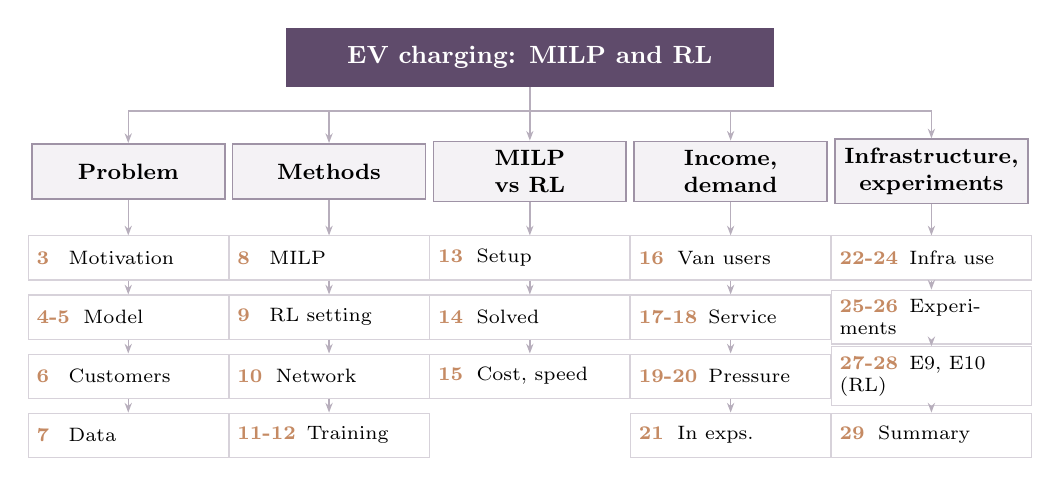
\begin{tikzpicture}[
 root/.style={fill=accP,text=white,minimum width=6.2cm,minimum height=.75cm,font=\small\bfseries},
 branch/.style={draw=accP!60,line width=.6pt,fill=accP!7,minimum width=2.45cm,minimum height=.7cm,font=\footnotesize\bfseries,align=center},
 leaf/.style={draw=accP!25,line width=.4pt,fill=white,text width=2.33cm,minimum height=.56cm,font=\scriptsize,align=left,inner xsep=3pt},
 arr/.style={-{Stealth[length=3.5pt]},accP!45,line width=.5pt}]
\node[root] (r) at (6.4,0) {EV charging: MILP and RL};
\foreach \x/\n/\t in {1.3/b1/{Problem},3.85/b2/{Methods},6.4/b3/{MILP\\vs RL},8.95/b4/{Income,\\demand},11.5/b5/{Infrastructure,\\experiments}}{
  \node[branch] (\n) at (\x,-1.45) {\t};
  \draw[arr] (r.south) -- ++(0,-.3) -| (\n.north);
}
\node[leaf] (a1) at (1.3,-2.55) {\textcolor{accA}{\bfseries 3}\;\; Motivation};
\node[leaf] (a2) at (1.3,-3.3)  {\textcolor{accA}{\bfseries 4-5}\; Model};
\node[leaf] (a3) at (1.3,-4.05) {\textcolor{accA}{\bfseries 6}\;\; Customers};
\node[leaf] (a4) at (1.3,-4.8)  {\textcolor{accA}{\bfseries 7}\;\; Data};
\node[leaf] (c1) at (3.85,-2.55) {\textcolor{accA}{\bfseries 8}\;\; MILP};
\node[leaf] (c2) at (3.85,-3.3)  {\textcolor{accA}{\bfseries 9}\;\; RL setting};
\node[leaf] (c3) at (3.85,-4.05) {\textcolor{accA}{\bfseries 10}\; Network};
\node[leaf] (c4) at (3.85,-4.8)  {\textcolor{accA}{\bfseries 11-12}\, Training};
\node[leaf] (d1) at (6.4,-2.55) {\textcolor{accA}{\bfseries 13}\; Setup};
\node[leaf] (d2) at (6.4,-3.3)  {\textcolor{accA}{\bfseries 14}\; Solved};
\node[leaf] (d3) at (6.4,-4.05) {\textcolor{accA}{\bfseries 15}\; Cost, speed};
\node[leaf] (e1) at (8.95,-2.55) {\textcolor{accA}{\bfseries 16}\; Van users};
\node[leaf] (e2) at (8.95,-3.3)  {\textcolor{accA}{\bfseries 17-18}\, Service};
\node[leaf] (e3) at (8.95,-4.05) {\textcolor{accA}{\bfseries 19-20}\, Pressure};
\node[leaf] (e4) at (8.95,-4.8)  {\textcolor{accA}{\bfseries 21}\; In exps.};
\node[leaf] (f1) at (11.5,-2.55) {\textcolor{accA}{\bfseries 22-24}\, Infra use};
\node[leaf] (f2) at (11.5,-3.3)  {\textcolor{accA}{\bfseries 25-26}\, Experiments};
\node[leaf] (f3) at (11.5,-4.05) {\textcolor{accA}{\bfseries 27-28}\, E9, E10 (RL)};
\node[leaf] (f4) at (11.5,-4.8)  {\textcolor{accA}{\bfseries 29}\; Summary};
\foreach \a/\b in {b1/a1,a1/a2,a2/a3,a3/a4,b2/c1,c1/c2,c2/c3,c3/c4,b3/d1,d1/d2,d2/d3,b4/e1,e1/e2,e2/e3,e3/e4,b5/f1,f1/f2,f2/f3,f3/f4}{\draw[arr] (\a) -- (\b);}
\end{tikzpicture}
\end{frame}

% ======================================================================= 3 motivation
\begin{frame}{Motivation}
\begin{itemize}
  \item Parked EVs request charging during a period $[0,T]$.
  \item Two ways to serve a request:
  \begin{itemize}
    \item \textbf{Station (FCS)}: the EV drives there, may queue, charges at 22\,kW.
    \item \textbf{Van (MCS)}: comes to the parked EV, charges at 30\,kW; scarce, dearer.
  \end{itemize}
  \item Customers value time and money differently:
  \begin{itemize}
    \item \textbf{Personal} owners are free while a van charges.
    \item \textbf{Commercial} cars (taxis) lose earnings every minute off the road.
  \end{itemize}
  \item \textbf{Questions}: who gets a station, who a van, in which order?\\ Can a learned policy match the optimum, fast?
\end{itemize}
\end{frame}

% ======================================================================= 4 problem setting
\begin{frame}{Problem model}
\begin{columns}[T]
\column{.55\textwidth}
\begin{itemize}
  \item \textbf{EV $i$}: request $r_i$, energy $E_i$, range $R_i$, segment $s_i$, income $\theta_i\in[0,1]$
  \item \textbf{Stations}: 12 $\times$ 2 guns, 22\,kW, one EV per gun at a time
  \item \textbf{Vans}: 5 from a depot; 30\,kW, 150\,kWh, $\le$ 6 EVs
  \item \textbf{Decide}: gun or van per EV, gun order, van routes, start times
\end{itemize}
\column{.42\textwidth}
\centering
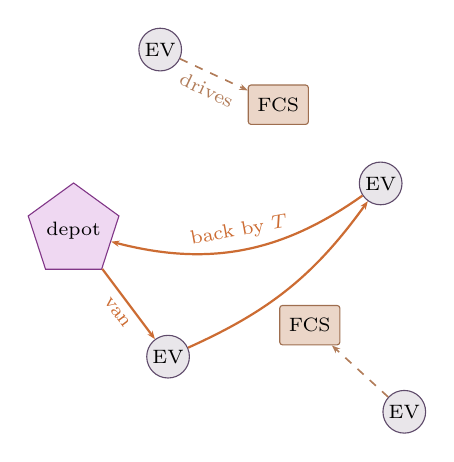
\begin{tikzpicture}[font=\scriptsize,
  ev/.style={circle,draw=accP,fill=cEV,inner sep=1.2pt,minimum size=5mm},
  st/.style={rectangle,rounded corners=1pt,draw=accA!80!black,fill=cFCS,minimum size=5mm},
  dp/.style={regular polygon,regular polygon sides=5,draw=gradPurple!70!black,fill=cDepot,minimum size=8.5mm,inner sep=0pt},
  drv/.style={-{Stealth[length=3pt]},accA!90!black,dashed,line width=.6pt},
  vn/.style={-{Stealth[length=3pt]},gradOrange!85!black,line width=.8pt}]
\node[dp] (d) at (0,0) {depot};
\node[st] (f1) at (2.6,1.6) {FCS};
\node[st] (f2) at (3.0,-1.2) {FCS};
\node[ev] (e1) at (1.1,2.3) {EV};
\node[ev] (e2) at (3.9,0.6) {EV};
\node[ev] (e3) at (1.2,-1.6) {EV};
\node[ev] (e4) at (4.2,-2.3) {EV};
\draw[drv] (e1) -- node[below,sloped]{drives} (f1);
\draw[drv] (e4) -- (f2);
\draw[vn] (d) -- node[below,sloped]{van} (e3);
\draw[vn] (e3) to[bend right=15] (e2);
\draw[vn] (e2) to[bend left=25] node[above,sloped]{back by $T$} (d);
\end{tikzpicture}
\end{columns}
\end{frame}

% ======================================================================= 5 objective
\begin{frame}{Objective and constraints}
\textbf{Minimise} operator cost + cost perceived by customers:
\[
Z=\underbrace{Z_1}_{\text{EV driving}}+\underbrace{Z_2}_{\text{van km}}+\underbrace{Z_3}_{\text{van dispatch}}
 +\underbrace{Z_4}_{\text{energy}}+\underbrace{Z_5}_{\text{tariff}\times\mu_i}+\underbrace{Z_6}_{\text{time}\times c^{a}_i}
\]
\textbf{Subject to}
\begin{itemize}
  \item each EV served once; a station only within range $R_i$
  \item one EV per gun at a time; station queue $\le W_i$
  \item vans: $\le$ 6 EVs, battery limit, back at the depot by $T$
  \item every EV fully charged by $T$
\end{itemize}
Segment and income act only through $\mu_i$, $c^{a}_i$, $W_i$: model size unchanged.
\end{frame}

% ======================================================================= 6 customer model
\begin{frame}{Customer model: segment and income}
\begin{columns}[T]
\column{.6\textwidth}
\scriptsize\setlength{\tabcolsep}{3.5pt}
\begin{tabular}{lrrrr}
\toprule
 & \multicolumn{2}{c}{personal} & \multicolumn{2}{c}{commercial}\\
parameter & $\theta=0$ & $\theta=1$ & $\theta=0$ & $\theta=1$\\
\midrule
money sensitivity $\mu$ & 1.5 & 0.5 & 1.5 & 0.5\\
driving $c^D$ (Rs/min) & 1.5 & 15 & 1.5 & 6\\
queueing $c^Q$ (Rs/min) & 2.5 & 25 & 2.0 & 7.5\\
station charging $c^C$ & 1.0 & 10 & 1.5 & 6\\
van wait + charging $c^V$ & 0.5 & 5 & 1.5 & 6\\
queue tolerance $W$ (min) & 60 & 15 & 40 & 15\\
\bottomrule
\end{tabular}

\vspace{1ex}
Tariffs: station 15\,Rs/kWh, van 25\,Rs/kWh.
\column{.37\textwidth}
\small
\begin{itemize}
  \item Linear in income $\theta$.
  \item Commercial: one downtime rate $\omega(\theta)$ for all time.
  \item 70\% of requests commercial.
  \item $\theta$: personal Beta(2.5,\,1), commercial Beta(3,\,5).
\end{itemize}
\end{columns}
\end{frame}

% ======================================================================= 7 data
\begin{frame}{Data: EV-Solomon instances}
\begin{itemize}
  \item 56 Solomon routing files, classes C1, C2, R1, R2, RC1, RC2.
  \item Customers $\to$ EVs; ready times $\to$ requests; demand $\to$ 10--40\,kWh.
  \item Stations at k-means centres; 15\% of EVs reachable only by van.
  \item Horizon $T$: short 230--1236\,min (type 1), long 960--3390\,min (type 2).
  \item Instance = file + first $n$ EVs, $n=10,\dots,100$: \textbf{560 instances}, shared by all methods.
\end{itemize}
\end{frame}

% ======================================================================= 8 MILP
\begin{frame}{Exact model (MILP) and baseline}
\begin{itemize}
  \item \textbf{MILP}: full model, Gurobi 13, 300\,s per instance, 32 cores; greedy warm start.
  \item Size at $n=100$: about 56\,000 binaries, 172\,000 constraints.
  \item \textbf{Greedy rule}: stranded EVs first, then by request time; each takes its cheapest feasible charger.
  \item \textbf{Checker}: every plan of every method is re-checked and its $Z$ recomputed.
\end{itemize}
\end{frame}

% ======================================================================= 9 RL formulation
\begin{frame}{RL formulation}
\begin{columns}[T]
\column{.5\textwidth}
\begin{itemize}
  \item \textbf{Episode}: build one plan for one instance.
  \item \textbf{State}: EVs placed or dropped; gun free times; van position, free time, battery, seats.
  \item \textbf{Action}: (EV $i$, charger $k$); $i$ joins $k$ at the earliest start.
\end{itemize}
\column{.5\textwidth}
\begin{itemize}
  \item \textbf{Mask}: range, queue $\le W_i$, done by $T$, van seat and battery.
  \item \textbf{Step cost}: $\Delta Z_{ik}$.
  \item \textbf{End}: all EVs placed or dropped.
  \item \textbf{Plan cost}: $L = Z + 10\,\sigma\cdot\text{dropped}$
\end{itemize}
\end{columns}
\end{frame}

% ======================================================================= 10 policy network
\begin{frame}{Policy network}
\centering
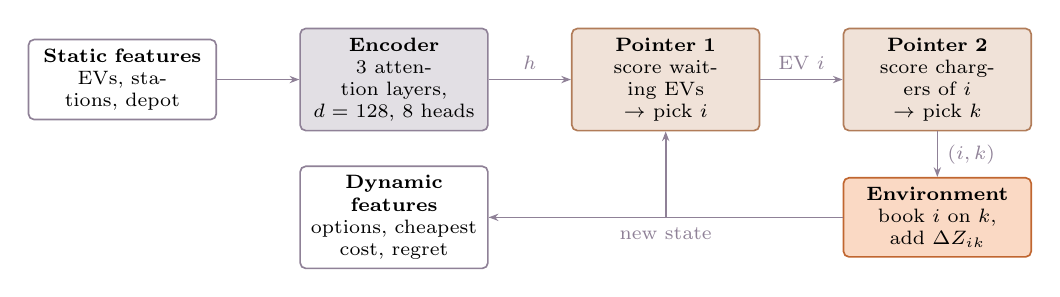
\begin{tikzpicture}[font=\scriptsize,
  bx/.style={draw=accP!70,fill=white,rounded corners=2pt,align=center,minimum height=.95cm,text width=2.15cm,line width=.6pt},
  enc/.style={bx,fill=cNet},
  ptr/.style={bx,fill=cPtr,draw=accA!90!black},
  envb/.style={bx,fill=cVan,draw=gradOrange!80!black},
  a/.style={-{Stealth[length=3.5pt]},accP!70,line width=.6pt}]
\node[bx] (in) at (0,0) {\textbf{Static features}\\ EVs, stations, depot};
\node[enc] (enc) at (3.45,0) {\textbf{Encoder}\\ 3 attention layers,\\ $d=128$, 8 heads};
\node[bx] (dyn) at (3.45,-1.75) {\textbf{Dynamic features}\\ options, cheapest cost, regret};
\node[ptr] (p1) at (6.9,0) {\textbf{Pointer 1}\\ score waiting EVs\\ $\to$ pick $i$};
\node[ptr] (p2) at (10.35,0) {\textbf{Pointer 2}\\ score chargers of $i$\\ $\to$ pick $k$};
\node[envb] (env) at (10.35,-1.75) {\textbf{Environment}\\ book $i$ on $k$, add $\Delta Z_{ik}$};
\draw[a] (in) -- (enc);
\draw[a] (enc) -- node[above]{$h$} (p1);
\draw[a] (p1) -- node[above]{EV $i$} (p2);
\draw[a] (dyn) -| (p1);
\draw[a] (p2) -- node[right]{$(i,k)$} (env);
\draw[a] (env) -- node[below]{new state} (dyn);
\end{tikzpicture}

\vspace{2ex}
\raggedright
\begin{itemize}
  \item Infeasible choices masked; $\log\pi(i,k)=\log\pi(i)+\log\pi(k\mid i)$.
  \item \Params{} parameters; works for any $n$, stations and vans.
\end{itemize}
\end{frame}

% ======================================================================= 11 training
\begin{frame}{RL training: REINFORCE with a shared baseline}
\begin{columns}[T]
\column{.56\textwidth}
\begin{algorithm}[H]
\caption{RL Training}
\For{epoch $=1$ \KwTo 500}{
  \For{batch $=1$ \KwTo 50}{
    Generate 32 random instances (same $n$)\;
    \eIf{first 500 batches (warm-up)}{
      copy the greedy rule: loss $=-\frac1n\log\pi_\theta(\text{rule plan})$\;
    }{
      8 sampled episodes per instance, costs $L_j$\;
      loss $=$ mean $A_j\log\pi_\theta(\text{plan}_j)$, $A_j=(L_j-\bar L)/\bar L$\;
    }
    Adam step on $\theta$ (gradient norm $\le 1$)\;
  }
  Validate against the greedy rule; keep the best $\theta$\;
}
\end{algorithm}
\column{.4\textwidth}
\small
\begin{itemize}
  \item Random initial weights.
  \item $\bar L$: mean cost of the 8 plans of an instance; no critic, no replay buffer.
  \item Early stop: 10 epochs without gain, after epoch 200.
  \item Test: 8 map rotations $\times$ (1 greedy + 64 sampled) plans; best kept.
\end{itemize}
\end{columns}
\end{frame}

% ======================================================================= 12 representative example
% Toy instance: 1 station (2 guns, 22 kW), 1 van (30 kW), 3 EVs. Delta Z values are exact for these inputs
% (formulation-4 coefficients); the network probabilities are illustrative.
\begin{frame}{Representative example: one step}
\centering
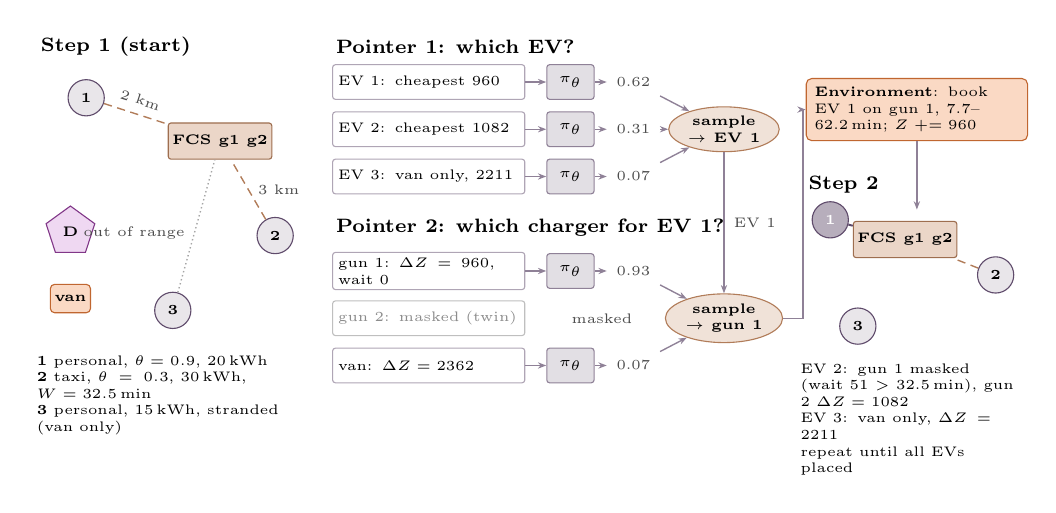
\begin{tikzpicture}[font=\scriptsize,
  ev/.style={circle,draw=accP,fill=cEV,inner sep=0.6pt,minimum size=4.6mm,font=\tiny\bfseries},
  evd/.style={ev,fill=accP!45,text=white},
  st/.style={rectangle,rounded corners=1pt,draw=accA!80!black,fill=cFCS,minimum height=4.6mm,inner sep=1.5pt,font=\tiny\bfseries},
  dp/.style={regular polygon,regular polygon sides=5,draw=gradPurple!70!black,fill=cDepot,minimum size=6.5mm,inner sep=0pt,font=\tiny\bfseries},
  van/.style={rectangle,rounded corners=1.5pt,draw=gradOrange!80!black,fill=cVan,minimum height=3.6mm,inner sep=1.5pt,font=\tiny\bfseries},
  opt/.style={accA!90!black,densely dashed,line width=.5pt},
  bad/.style={black!35,densely dotted,line width=.5pt},
  inp/.style={draw=accP!50,fill=white,rounded corners=1pt,minimum height=4.4mm,inner sep=2pt,align=left,text width=2.3cm,font=\tiny},
  nn/.style={draw=accP!70,fill=cNet,rounded corners=1pt,minimum width=6mm,minimum height=4.4mm,inner sep=0pt,font=\tiny\bfseries},
  pick/.style={ellipse,draw=accA!90!black,fill=cPtr,inner sep=1pt,font=\tiny\bfseries,align=center},
  envb/.style={draw=gradOrange!80!black,fill=cVan,rounded corners=2pt,align=left,text width=2.6cm,inner sep=3pt,font=\tiny},
  a/.style={-{Stealth[length=3pt]},accP!70,line width=.5pt},
  lab/.style={font=\tiny,text=black!70}]
% ---------------- left: instance at the start of the episode
\node[font=\scriptsize\bfseries,anchor=west] at (-0.2,0.45) {Step 1 (start)};
\node[dp] (d) at (0.3,-1.9) {D};
\node[st] (s) at (2.2,-0.75) {FCS g1 g2};
\node[van] (v) at (0.3,-2.75) {van};
\node[ev] (e1) at (0.5,-0.2) {1};
\node[ev] (e2) at (2.9,-1.95) {2};
\node[ev] (e3) at (1.6,-2.9) {3};
\draw[opt] (e1) -- node[lab,above,sloped]{2 km} (s);
\draw[opt] (e2) -- node[lab,right]{3 km} (s);
\draw[bad] (e3) -- node[lab,left,pos=.45]{out of range} (s);
\node[align=left,anchor=north west,font=\tiny,text width=3.1cm] at (-0.25,-3.35)
 {\textbf{1} personal, $\theta=0.9$, 20\,kWh\\ \textbf{2} taxi, $\theta=0.3$, 30\,kWh, $W=32.5$\,min\\ \textbf{3} personal, 15\,kWh, stranded (van only)};
% ---------------- middle top: pointer 1 (choose the EV)
\node[font=\scriptsize\bfseries,anchor=west] at (3.55,0.45) {Pointer 1: which EV?};
\foreach \k/\y/\t/\p in {1/0/{EV 1: cheapest 960}/0.62, 2/-0.6/{EV 2: cheapest 1082}/0.31, 3/-1.2/{EV 3: van only, 2211}/0.07}{
  \node[inp] (i\k) at (4.85,\y) {\t};
  \node[nn] (n\k) at (6.65,\y) {$\pi_\theta$};
  \node[lab] (p\k) at (7.45,\y) {\p};
  \draw[a] (i\k) -- (n\k); \draw[a] (n\k) -- (p\k);
}
\node[pick] (k1) at (8.6,-0.6) {sample\\ $\to$ EV 1};
\foreach \k in {1,2,3}{\draw[a] (p\k) -- (k1);}
% ---------------- middle bottom: pointer 2 (choose the charger of EV 1)
\node[font=\scriptsize\bfseries,anchor=west] at (3.55,-1.85) {Pointer 2: which charger for EV 1?};
\node[inp] (j1) at (4.85,-2.4) {gun 1: $\Delta Z=960$, wait 0};
\node[inp,draw=black!25,text=black!45] (j2) at (4.85,-3.0) {gun 2: masked (twin)};
\node[inp] (j3) at (4.85,-3.6) {van: $\Delta Z=2362$};
\foreach \k/\y/\p in {1/-2.4/0.93, 3/-3.6/0.07}{
  \node[nn] (m\k) at (6.65,\y) {$\pi_\theta$};
  \node[lab] (q\k) at (7.45,\y) {\p};
  \draw[a] (j\k) -- (m\k); \draw[a] (m\k) -- (q\k);
}
\node[lab] at (7.05,-3.0) {masked};
\node[pick] (k2) at (8.6,-3.0) {sample\\ $\to$ gun 1};
\draw[a] (q1) -- (k2); \draw[a] (q3) -- (k2);
\draw[a] (k1) -- node[lab,right]{EV 1} (k2);
% ---------------- right: environment update and the next state
\node[envb] (env) at (11.05,-0.35) {\textbf{Environment}: book EV 1 on gun 1, 7.7--62.2\,min; $Z \mathrel{+}= 960$};
\draw[a] (k2.east) -- ++(0.25,0) |- (env.west);
\node[font=\scriptsize\bfseries,anchor=west] at (9.55,-1.3) {Step 2};
\node[st] (s2) at (10.9,-2.0) {FCS g1 g2};
\node[evd] (f1) at (9.95,-1.75) {1};
\node[ev] (f2) at (12.05,-2.45) {2};
\node[ev] (f3) at (10.3,-3.1) {3};
\draw[accP,line width=.7pt] (f1) -- (s2);
\draw[opt] (f2) -- (s2);
\draw[a] (env.south) -- (11.05,-1.62);
\node[align=left,anchor=north west,font=\tiny,text width=2.75cm] at (9.45,-3.45)
 {EV 2: gun 1 masked (wait 51 $>$ 32.5\,min), gun 2 $\Delta Z=1082$\\ EV 3: van only, $\Delta Z=2211$\\ repeat until all EVs placed};
\end{tikzpicture}

\vspace{-.3ex}
{\tiny $\Delta Z$ in Rs, exact for this toy instance; van cost includes 1500 dispatch; probabilities illustrative.}
\end{frame}

% ======================================================================= 13 setup
\begin{frame}{Experimental setup}
\begin{columns}[T]
\column{.5\textwidth}
\small
\begin{tabular}{ll}
\toprule
item & value\\
\midrule
instances & 560\\
MILP & Gurobi 13, 300\,s, 32 cores\\
RL training & \TrainMin{} min, one GPU\\
RL epochs & \TrainEpochs{} (best \BestEpoch)\\
RL test & 520 plans per instance\\
variants & 15 MILP + RL, 6 RL only\\
\bottomrule
\end{tabular}
\column{.46\textwidth}
\small
\textbf{Experiments} (one input changed)
\begin{itemize}
  \item E5: value of charging time $\pm25\%$
  \item E6: money sensitivity $\pm25\%$
  \item E1: van tariff 15 or 35 Rs/kWh
  \item E2: 3 or 7 vans; 4 or 8 seats
  \item E8: van battery 200 kWh
  \item E9 (RL only): 1 or 4 guns; 11 or 44 kW
  \item E10 (RL only): energy per EV $\times$0.75, $\times$1.25
\end{itemize}
\end{columns}
\end{frame}

% ======================================================================= 13 solved instances
\begin{frame}{Results: solved instances}
\begin{columns}[T]
\column{.55\textwidth}
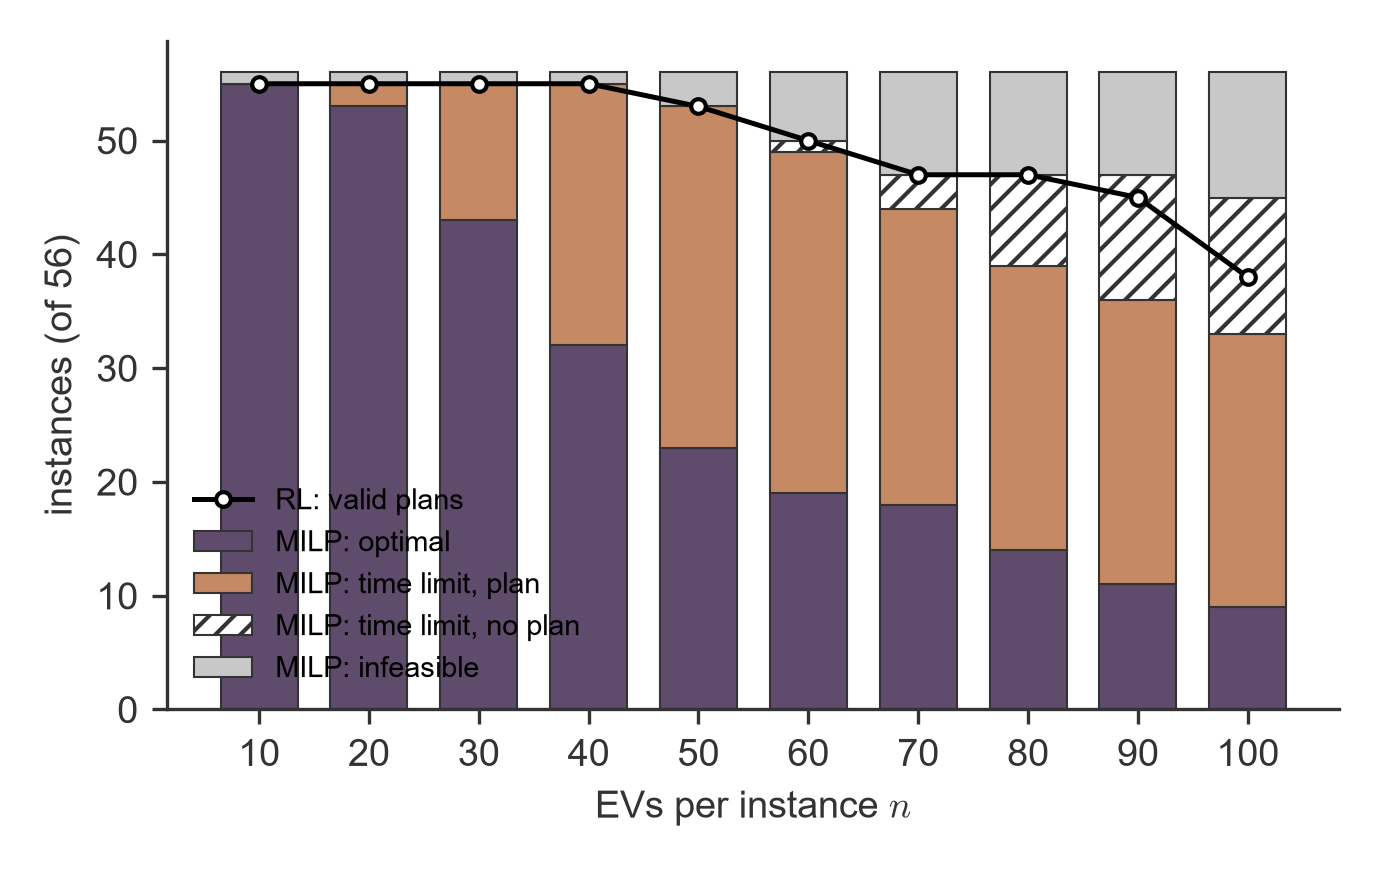
\includegraphics[width=\textwidth]{figures/outcome.png}
\column{.42\textwidth}
\small
\begin{itemize}
  \item MILP: \NOpt{} optimal, \NTL{} time-limit plans, \NNoPlan{} no plan, \NInf{} infeasible.
  \item Infeasibility comes from the data (short horizons R1, RC1).
  \item RL: \NValidR{} valid plans, \RlOnly{} where the MILP has none.
  \item RL never misses an instance the MILP solves.
\end{itemize}
\end{columns}
\end{frame}

% ======================================================================= 14 cost and speed
\begin{frame}{Results: cost and speed}
\begin{columns}[T]
\column{.55\textwidth}
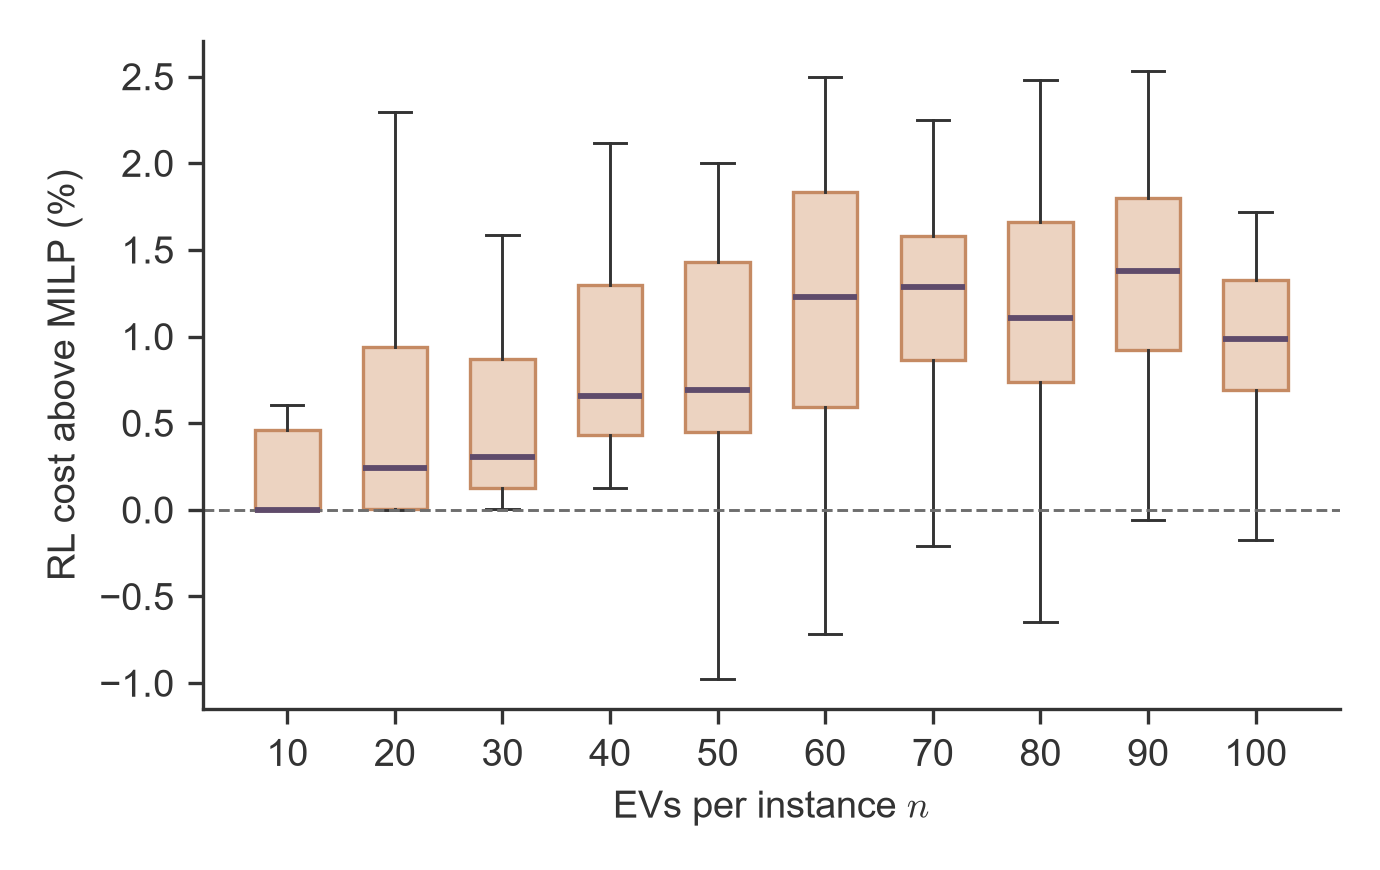
\includegraphics[width=\textwidth]{figures/gap.png}
\column{.42\textwidth}
\small
\begin{tabular}{lrr}
\toprule
 & MILP & RL\\
\midrule
valid plans & \NValidM & \NValidR\\
above MILP & -- & \GapMean\%\\
\quad median & -- & \GapMed\%\\
time & \TimeM\,s & \TimeR\,s\\
\bottomrule
\end{tabular}

\vspace{1ex}
\begin{itemize}
  \item \NPaired{} paired instances; RL beats the MILP's time-limit plan in \RlBetter.
  \item RL is about \Speed{}$\times$ faster.
\end{itemize}
\end{columns}
\end{frame}

% ======================================================================= 16 who gets a van
\begin{frame}{Who gets a van: segment and income}
\begin{columns}[T]
\column{.55\textwidth}
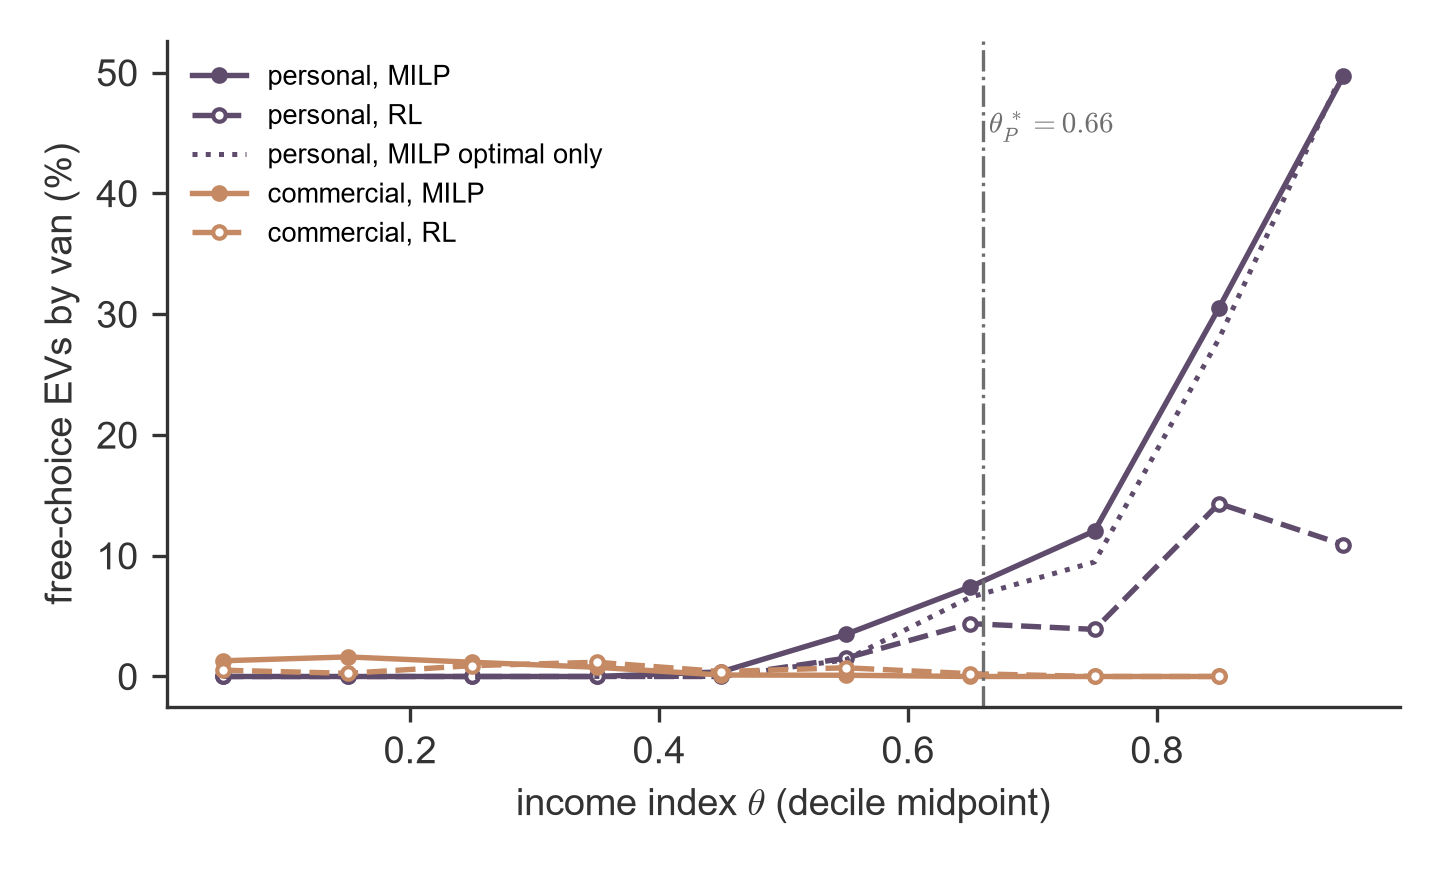
\includegraphics[width=\textwidth]{figures/van_decile.png}
\column{.42\textwidth}
\small
\begin{itemize}
  \item Personal: \VanPersonalMilp\% (MILP), \VanPersonalRl\% (RL).
  \item Optimal plans: \VanPersOptBelowFour\% below $\theta=0.4$, \VanPersOptTop\% in the top decile.
  \item Theory: $\theta^*_P=\ThetaStarP$; the step is there.
  \item Taxis: \VanCommercialMilp\%. A van costs \DeltaComOne{} Rs more even at $\theta=1$, unless the queue is $\ge$\QueueNeedCom{} min.
  \item All \NComVan{} taxi van users: time-limit plans, wait \ComVanWait{} min.
\end{itemize}
\end{columns}
\end{frame}

% ======================================================================= 17 service by segment x income
\begin{frame}{Service by segment and income}
\begin{columns}[T]
\column{.58\textwidth}
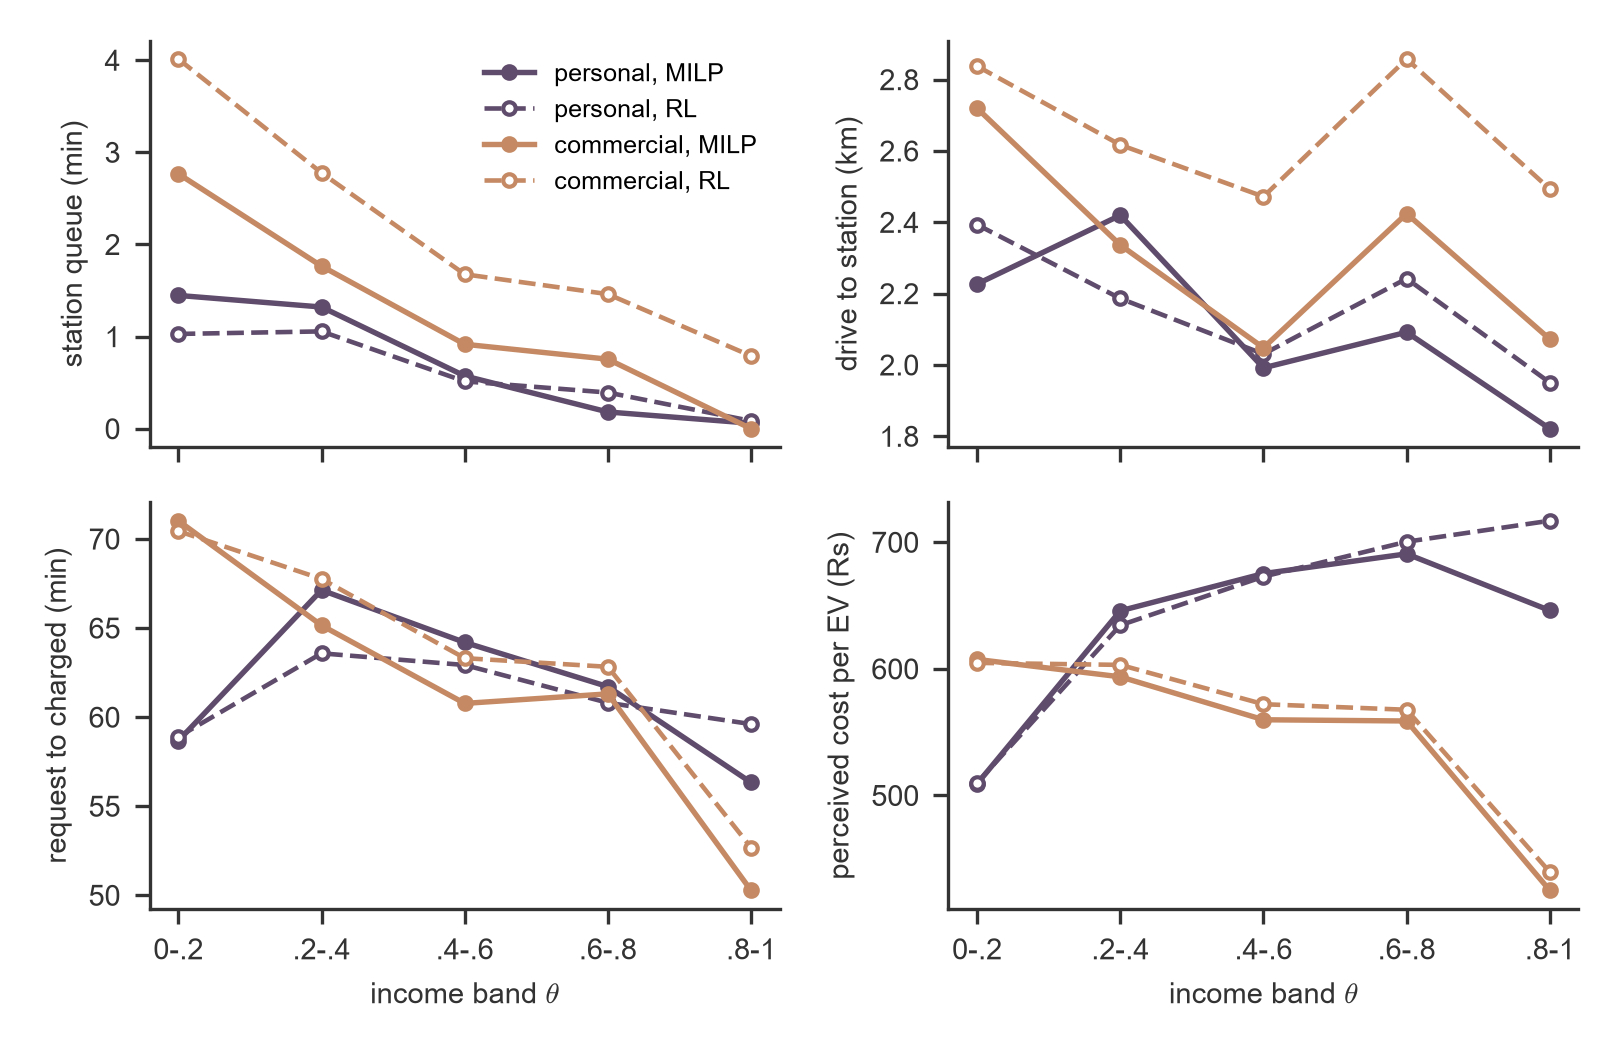
\includegraphics[width=\textwidth]{figures/seg_income.png}
\column{.39\textwidth}
\small
\begin{itemize}
  \item Poorer EVs queue longer and drive farther; taxis most.
  \item Rich personal owners: almost no queue, shortest drive, often a van.
  \item Perceived cost rises with income for personal owners (time valued), falls for taxis.
  \item RL: same shape, longer taxi queues.
\end{itemize}
\vspace{.5ex}
\scriptsize Station users; paired instances; MILP solid, RL dashed.
\end{columns}
\end{frame}

% ======================================================================= 18 who queues, who pays
\begin{frame}{Who queues and who pays}
\begin{columns}[T]
\column{.47\textwidth}
\scriptsize
\textbf{Station users vs queue minutes (\%)}\\[.5ex]
\setlength{\tabcolsep}{4pt}
\begin{tabular}{lrrrr}
\toprule
 & \multicolumn{2}{c}{MILP} & \multicolumn{2}{c}{RL}\\
group & users & queue & users & queue\\
\midrule
\TabQueueShare
\bottomrule
\end{tabular}
\column{.51\textwidth}
\scriptsize
\textbf{Per EV (Rs): paid, perceived (MILP, RL)}\\[.5ex]
\setlength{\tabcolsep}{2.4pt}
\begin{tabular}{lrrrrrr}
\toprule
 & \multicolumn{3}{c}{personal} & \multicolumn{3}{c}{commercial}\\
band & paid & M & R & paid & M & R\\
\midrule
\TabEquity
\bottomrule
\end{tabular}

\vspace{1ex}
\small
\begin{itemize}
  \item Queueing: taxis \QShareComM\% (users \QUserComM\%); $\theta<0.4$: \QSharePoorM\% (users \QUserPoorM\%).
  \item Time in perceived cost: personal \TimeSharePers\%, taxi \TimeShareCom\%.
\end{itemize}
\end{columns}
\end{frame}

% ======================================================================= 19 demand pressure: definition
\begin{frame}{Demand pressure: definition and effect}
\small
For EV $i$: \ window $w=$ mean station charging time of the instance's EVs (\PressWinMin--\PressWinMax{} min),
\[
\text{load}_i=\#\{\,j:\ r_i-w\le r_j\le r_i\,\},\qquad
\text{pressure}_i=\frac{\text{load}_i}{24\text{ guns}+5\text{ vans}}.
\]
Data only (no plan). Terciles over all 560 instances: low $\le\PressCutLo$ ($\le\PressLoadLo$ requests), high $>\PressCutHi$ ($>\PressLoadHi$).

\vspace{.5ex}
\scriptsize
\begin{tabular}{lrrrrrrrrr}
\toprule
 & & \multicolumn{4}{c}{free-choice EVs by van (\%)} & \multicolumn{4}{c}{station queue (min)}\\
 & EVs & \multicolumn{2}{c}{personal} & \multicolumn{2}{c}{taxi} & \multicolumn{2}{c}{personal} & \multicolumn{2}{c}{taxi}\\
pressure & (\%) & MILP & RL & MILP & RL & MILP & RL & MILP & RL\\
\midrule
\TabPress
\bottomrule
\end{tabular}
\end{frame}

% ======================================================================= 20 demand pressure: where congestion happens
\begin{frame}{Demand pressure: where congestion happens}
\begin{columns}[T]
\column{.55\textwidth}
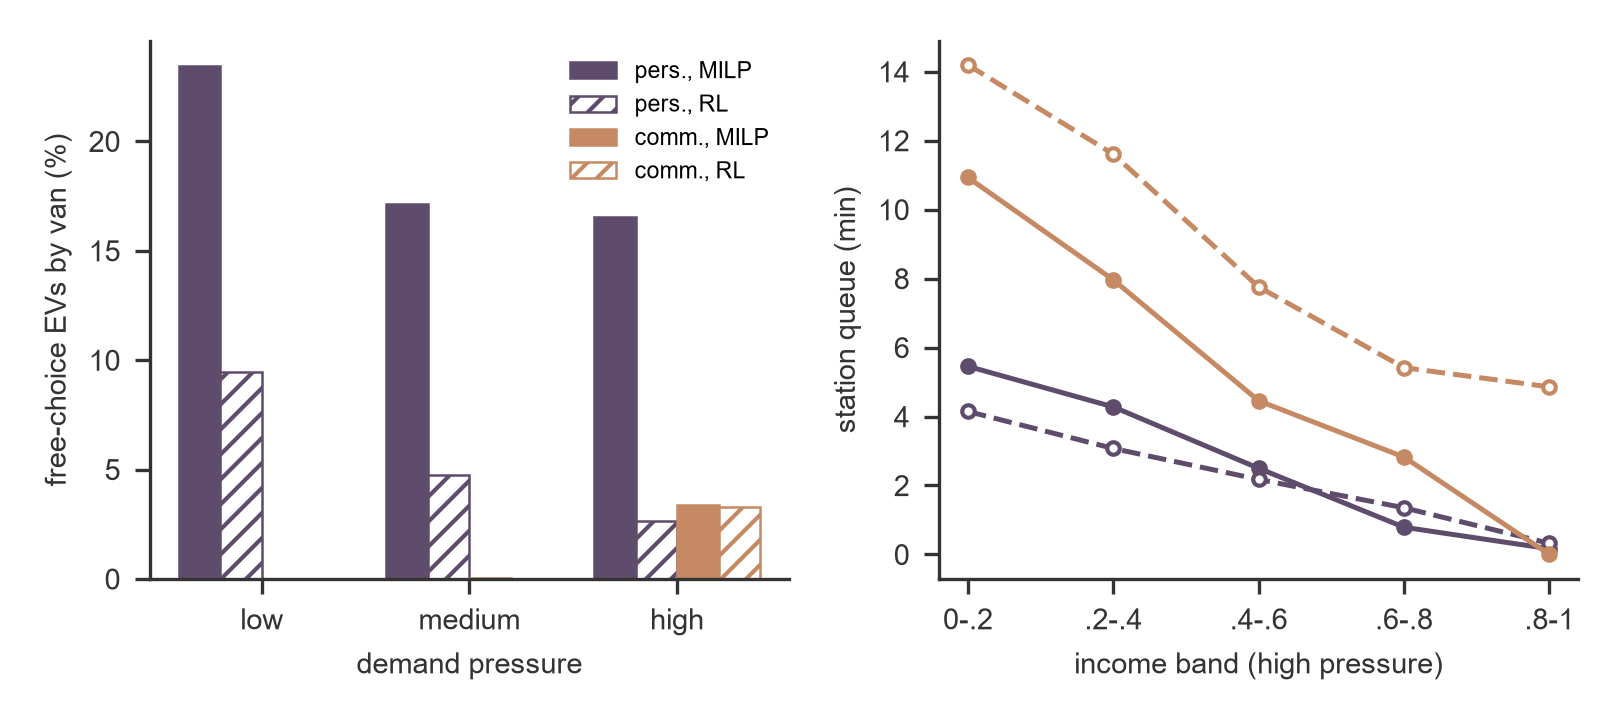
\includegraphics[width=\textwidth]{figures/pressure.png}
\column{.42\textwidth}
\small
\begin{itemize}
  \item Queued: \QueuedLoM\% / \QueuedMedM\% / \QueuedHiM\% (low / med / high).
  \item Taxis take vans only at high pressure (\VanComHiM\%).
  \item Personal vans fall: \VanPersLoM\% $\to$ \VanPersHiM\%.
  \item $\ge$ half the guns busy at request: \BusyHalfLoM\% low, \BusyHalfHiM\% high.
  \item Model's peak label (load $>$ median) misleads: \OffpeakHigh\% ``off-peak'' EVs are high pressure.
\end{itemize}
\end{columns}
\end{frame}

% ======================================================================= 21 pressure in the experiments
\begin{frame}{Demand pressure in the experiments}
\begin{columns}[T]
\column{.6\textwidth}
\scriptsize
\textbf{Change vs baseline, paired instances}\\[.5ex]
\setlength{\tabcolsep}{4pt}
\begin{tabular}{lrrrrr}
\toprule
 & \multicolumn{4}{c}{van share (points)} & queue\\
 & \multicolumn{2}{c}{personal, MILP} & \multicolumn{2}{c}{taxi, high} & taxi, high\\
variant & low & high & MILP & RL & (min)\\
\midrule
\TabExpPress
\bottomrule
\end{tabular}
\column{.37\textwidth}
\small
\begin{itemize}
  \item Cheap vans ($p^M$ 15) help personal owners off-peak (\PMLoPersLowM{} pts) more than at peak (\PMLoPersHighM).
  \item Prediction ``higher $\omega$ pushes taxis to vans at peak'': not seen (\OmegaHiComHighM{} MILP, \OmegaHiComHighR{} RL).
  \item 7 vans: fleet use \VansSevenFleet{} pts, taxis at peak \VansSevenComHigh.
  \item E9, E10 (RL only): on the station-capacity slides.
\end{itemize}
\end{columns}
\end{frame}

% ======================================================================= 22 infrastructure: guns
\begin{frame}{Infrastructure: stations and guns}
\begin{columns}[T]
\column{.55\textwidth}
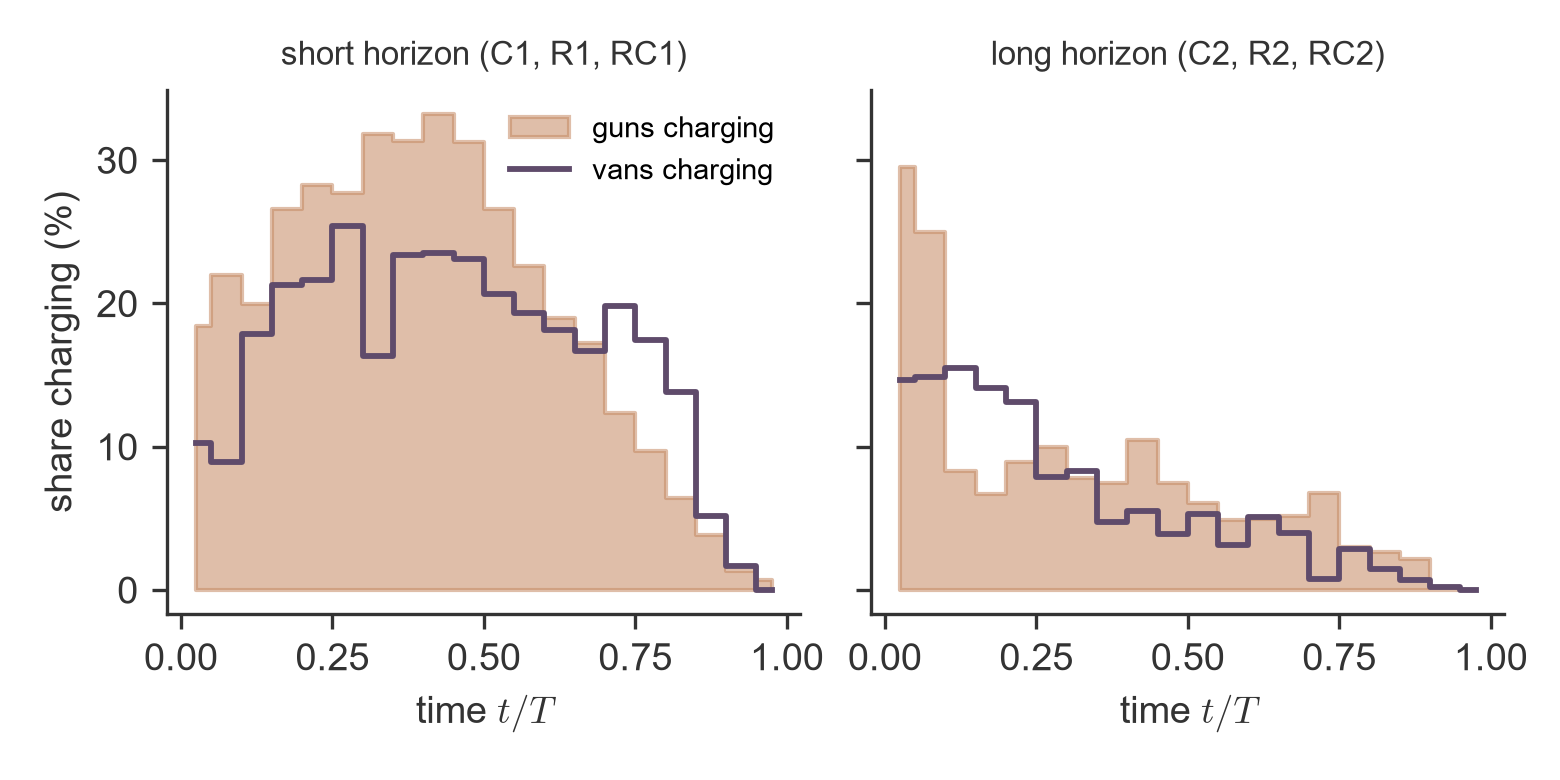
\includegraphics[width=\textwidth]{figures/busy.png}

\scriptsize Share of guns and vans charging over time (MILP).
\column{.42\textwidth}
\small
\begin{itemize}
  \item Gun busy over $[0,T]$: \GunUtilMilp\% (MILP), \GunUtilRl\% (RL); \GunUtilShort\% short, \GunUtilLong\% long horizons.
  \item Per gun: 90th pct \GunPninetyM\%, max \GunMaxM\%; \GunsNeverM\% never used.
  \item Idle guns per plan: \IdleGunsMilp{} (MILP), \IdleGunsRl{} (RL) of 24.
  \item Peak concurrency: \PeakGunsM{} guns (\PeakGunsHundredM{} at $n=100$); all 24 in \AllGunsBusyPlans{} plans.
\end{itemize}
\end{columns}
\end{frame}

% ======================================================================= 23 infrastructure: vans
\begin{frame}{Infrastructure: vans}
\begin{columns}[T]
\column{.58\textwidth}
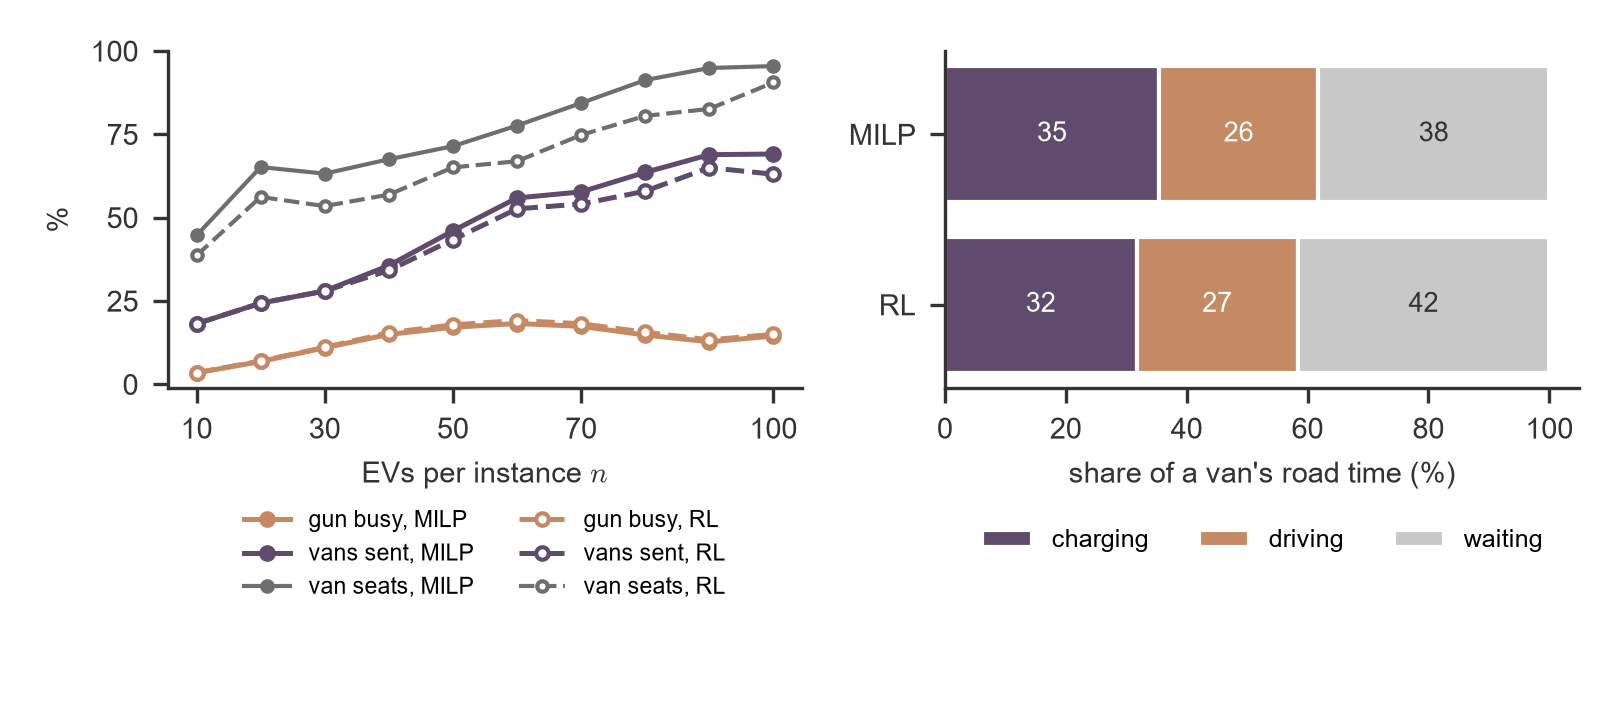
\includegraphics[width=\textwidth]{figures/infra_n.png}
\column{.39\textwidth}
\small
\begin{itemize}
  \item Vans sent: \FleetMilp\% (MILP), \FleetRl\% (RL).
  \item Seats: \SeatsMilp\% vs \SeatsRl\%; full vans \VansFullM\% vs \VansFullR\%.
  \item Battery drawn: \BattMilp\% vs \BattRl\%.
  \item Van energy: \VanDelivShare\% to EVs, \VanLossShare\% transfer loss, \VanDrvEShare\% driving.
  \item RL: fewer, emptier vans (\NVansR{} vs \NVansM).
\end{itemize}
\end{columns}
\end{frame}

% ======================================================================= 24 infrastructure by family
\begin{frame}{Infrastructure by family}
\scriptsize
\setlength{\tabcolsep}{4pt}
\begin{tabular}{lrrrrrrrrrrr}
\toprule
 & & \multicolumn{2}{c}{gun busy (\%)} & idle & peak & \multicolumn{2}{c}{vans sent (\%)} & \multicolumn{2}{c}{seats (\%)} & \multicolumn{2}{c}{van energy (\%)}\\
family & $T$ & MILP & RL & guns & guns & MILP & RL & MILP & RL & MILP & RL\\
\midrule
\TabInfraFam
\bottomrule
\end{tabular}

\vspace{1.5ex}
\small
\begin{itemize}
  \item Short horizons (R1, RC1): guns busiest; vans run out of time, seats half used.
  \item Long horizons (C2, R2): guns almost idle; vans run out of seats.
  \item Peak guns and idle guns from MILP plans; all values mean per plan / van.
\end{itemize}
\end{frame}

% ======================================================================= 25 experiments: cost
\begin{frame}{Experiments: cost}
\scriptsize
\renewcommand{\arraystretch}{.82}
\begin{tabular}{lrrrrrr}
\toprule
 & MILP valid & \multicolumn{3}{c}{MILP change (\%)} & \multicolumn{2}{c}{RL $\Delta Z$ (\%)}\\
variant & (new / lost) & $Z$ & operator & customer & zero-shot & retrained\\
\midrule
\TabExpCost
\bottomrule
\end{tabular}

\vspace{.6ex}
\scriptsize Means over paired instances; RL tracks the MILP's $\Delta Z$ with or without retraining. E9, E10 are RL only (next slides).
\end{frame}

% ======================================================================= 26 experiments: who and what
\begin{frame}{Experiments: who and what changes}
\scriptsize
\renewcommand{\arraystretch}{.82}
\setlength{\tabcolsep}{4.5pt}
\begin{tabular}{lrrrrrrrr}
\toprule
 & \multicolumn{3}{c}{van share (points)} & \multicolumn{5}{c}{MILP utilisation (points)}\\
variant & personal & taxi & personal RL & gun busy & vans sent & seats & battery & van energy\\
\midrule
\TabExpWho
\bottomrule
\end{tabular}

\vspace{.6ex}
\scriptsize Tariff and personal $c^{C,1}$ move who gets vans; fleet, seats and battery change only van use.
\end{frame}

% ======================================================================= 27 E9, E10 (RL only): cost and utilisation
\begin{frame}{Station capacity and charging demand (RL only)}
\scriptsize
\textbf{E9, E10: retrained RL vs RL baseline, paired instances} (no MILP run)\\[.4ex]
\renewcommand{\arraystretch}{.9}
\begin{tabular}{lrrrrrr}
\toprule
 & RL valid & \multicolumn{3}{c}{change (\%)} & \multicolumn{2}{c}{van share (points)}\\
variant & (new / lost) & $Z$ & operator & customer & personal & taxi\\
\midrule
\TabRLOnlyCost
\bottomrule
\end{tabular}

\vspace{1ex}
\begin{tabular}{lrrrrrr}
\toprule
 & & gun busy & idle guns & \multicolumn{3}{c}{change (points)}\\
variant & guns & \% (change) & (change) & vans sent & seats & van energy\\
\midrule
\TabRLOnlyUtil
\bottomrule
\end{tabular}
\end{frame}

% ======================================================================= 28 E9, E10 (RL only): what moves
\begin{frame}{E9, E10: what moves (RL only)}
\begin{columns}[T]
\column{.52\textwidth}
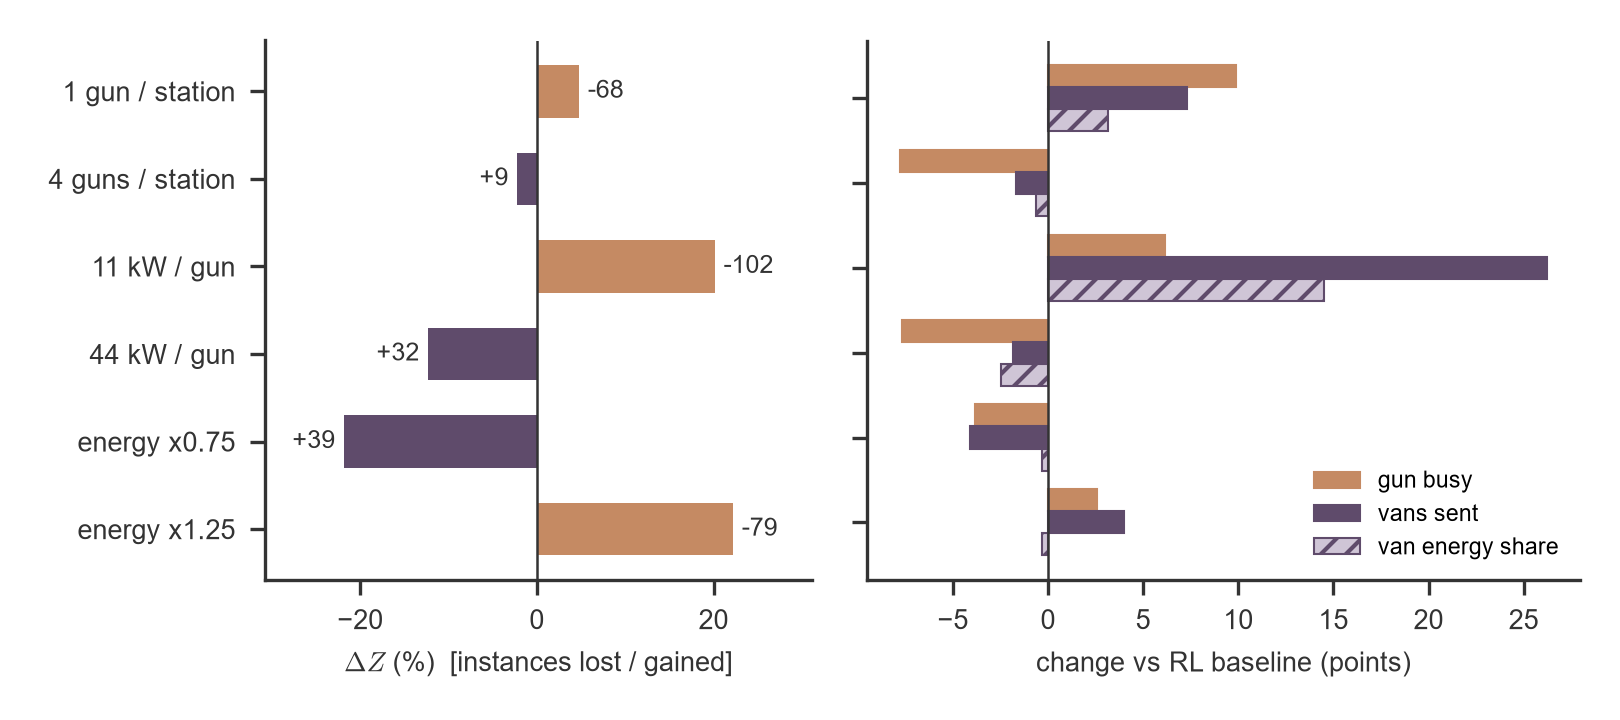
\includegraphics[width=\textwidth]{figures/rl_only.png}

\scriptsize
\begin{itemize}
  \item 11\,kW: \RLLostPowerEleven{} lost, $Z$ \RLdZPowerEleven\%, personal vans \RLVanPPowerEleven{} pts.
  \item 1 gun: \RLLostGunsOne{} lost, $Z$ \RLdZGunsOne\%, peak queue \RLQHighBaseGunsOne{} $\to$ \RLQHighGunsOne{} min.
  \item 44\,kW: \RLNewPowerFortyFour{} gained, $Z$ \RLdZPowerFortyFour\%; energy $\pm25\%$: $Z$ \RLdZDemandLow\% / \RLdZDemandHigh\%.
\end{itemize}
\column{.46\textwidth}
\scriptsize
\textbf{Demand pressure: change vs RL baseline}\\[.4ex]
\setlength{\tabcolsep}{2pt}
\begin{tabular}{lrrrr}
\toprule
 & \multicolumn{3}{c}{van share (pts)} & $\Delta$\\
variant & pers.\,lo & pers.\,hi & taxi hi & queue\\
\midrule
\TabRLOnlyPress
\bottomrule
\end{tabular}

\vspace{.6ex}
Queue: station users at high pressure (min).
\end{columns}
\end{frame}

% ======================================================================= 29 summary
\begin{frame}{Summary}
\begin{itemize}
  \item MILP: \NOpt{} of 560 optimal in 300\,s; RL: \NValidR{} valid plans, \GapMean\% above, \Speed{}$\times$ faster.
  \item Income decides vans for personal owners ($\theta^*_P=\ThetaStarP$); taxis stay at stations.
  \item Taxis are \QUserComM\% of station users but do \QShareComM\% of the queueing.
  \item Queues are a high-pressure effect (\QueueAllHiM{} min vs \QueueAllLoM); at peak, vans go to poor taxis.
  \item Guns busy \GunUtilMilp\% on average, vans charge only \ChargeMilp\% of the time; bursts, not capacity, bind.
  \item RL only: station power matters most (11\,kW: $Z$ \RLdZPowerEleven\%, \RLLostPowerEleven{} instances lost).
  \item Next: calibrate values of time, evening demand peak, 200-EV instances.
\end{itemize}
\end{frame}

\end{document}
